\documentclass[10pt,twoside]{article}

\usepackage[T1]{fontenc}
\usepackage[utf8]{inputenc}
\usepackage{newtxtext}
\usepackage{mathtools,amsthm}
\usepackage{newtxmath}
\usepackage[margin=0.78in,top=0.62in,bottom=0.70in]{geometry}
\usepackage{microtype}
\usepackage{xcolor}
\usepackage{booktabs,tabularx,array}
\usepackage{enumitem}
\usepackage{titlesec}
\usepackage{caption}
\usepackage{tikz}
\usepackage{pgfplots}
\usepackage[numbers,sort&compress]{natbib}
\usepackage[colorlinks=true,allcolors=MidnightBlue]{hyperref}
\usepackage[nameinlink,noabbrev]{cleveref}

\pgfplotsset{compat=1.18}

\definecolor{MidnightBlue}{HTML}{16324F}
\definecolor{SignalBlue}{HTML}{277DA1}
\definecolor{WarmGold}{HTML}{D69E2E}
\definecolor{SoftRed}{HTML}{C8553D}
\definecolor{Ink}{HTML}{20262E}
\definecolor{Mist}{HTML}{F2F5F7}
\definecolor{RuleGray}{HTML}{CBD5DE}

\color{Ink}
\hypersetup{pdfauthor={Jonathan R. Landers},pdftitle={Where the Signal Lives}}
\setlength{\parindent}{1.05em}
\setlength{\parskip}{0.15em}
\setlist{nosep,leftmargin=1.35em}
\captionsetup{font=small,labelfont={bf,color=MidnightBlue},skip=5pt}
\titleformat{\section}{\Large\bfseries\color{MidnightBlue}}{}{0pt}{}
\titleformat{\subsection}{\large\bfseries\color{MidnightBlue}}{}{0pt}{}
\titlespacing*{\section}{0pt}{1.15em}{0.42em}
\titlespacing*{\subsection}{0pt}{0.9em}{0.28em}

\pagestyle{plain}

\newtheoremstyle{noteplain}
  {0.65em}{0.65em}{\itshape}{} {\bfseries\color{MidnightBlue}}{.}{0.5em}{}
\theoremstyle{noteplain}
\newtheorem{theorem}{Theorem}
\newtheorem{lemma}[theorem]{Lemma}
\newtheorem{proposition}[theorem]{Proposition}
\newtheorem{corollary}[theorem]{Corollary}
\theoremstyle{definition}
\newtheorem{definition}[theorem]{Definition}
\renewcommand{\qedsymbol}{\color{SignalBlue}$\blacksquare$}

\newcommand{\R}{\mathbb{R}}
\newcommand{\one}{\mathbf{1}}
\newcommand{\E}{\mathbb{E}}
\newcommand{\Prb}{\mathbb{P}}
\newcommand{\KL}{D_{\mathrm{KL}}}
\newcommand{\Ber}{\operatorname{Ber}}
\newcommand{\ind}{\mathbf{1}}

\newcommand{\takeaway}[1]{%
  \par\medskip
  \noindent\fcolorbox{SignalBlue}{Mist}{%
    \begin{minipage}{0.94\linewidth}
      \small\textbf{Takeaway.} #1
    \end{minipage}}
  \par\medskip
}

\begin{document}

\begin{center}
  {\fontsize{25}{29}\selectfont\bfseries\color{MidnightBlue}Where the Signal Lives}\par\vspace{0.25em}
  {\Large Bounded-context prediction in Hadamard representatives}\par\vspace{0.85em}
  {\normalsize Jonathan R. Landers}\par\vspace{0.25em}
  {\small August 2026}
\end{center}

\vspace{0.35em}
\noindent\colorbox{Mist}{%
\begin{minipage}{0.965\linewidth}
\small
\textbf{Abstract.}
A Hadamard matrix is globally rigid: every pair of rows is orthogonal.  Does a reader who sees only the previous few signs gain any useful information about the next one?  We make that question precise for row-wise traversal and separate three possible sources of predictability: normalization, row balance, and the ordering of a chosen representative.  Exact arguments show that one-step prediction is neutral, that balance alone creates higher-order dependence, and that bounded-context statistics need not be invariant under Hadamard equivalence.  We then fit smoothed context models on complete equivalence classes and evaluate them on held-out classes from the McKay catalog.  Across 20 paired repetitions at orders $24$ and $28$, catalog representatives are strongly predictable, but almost all of the gain vanishes after equivalence-preserving row and column permutations.  At order $28$ and context length $8$, the gain over a fair coin is $0.13935$ nats for catalog representatives, $0.03047$ for permuted equivalents, and $0.03033$ for balanced rows.  The residual permuted-minus-balanced contrast is $0.00014$ with a 95\% interval containing zero.  The local signal is therefore real, transferable, and predominantly representational.  This first result locates the signal; the larger program asks what survives representation, what predicts a region, and whether such prediction actually improves exact search.
\end{minipage}}

\section{Orthogonality is a global promise; prediction is a local wager}

A Hadamard matrix looks least random when viewed all at once.  Its rows form an orthogonal basis, its normalized nonfirst rows are perfectly balanced, and a single wrong sign can destroy feasibility.  Yet a bounded observer does not see the whole matrix.  The observer sees a short row-wise context and must wager on the next sign.  Global rigidity and local predictability are therefore different questions.

The project surrounding this note is organized by one sentence:

\begin{quote}
\centering\itshape
Hadamard matrices reveal how global order can make local summaries predictable without making local decisions wise: the constraint state tells us what the next region should look like, but not which plausible region can belong to a complete whole.
\end{quote}

This first note asks where the local information lives.  Is it intrinsic to a Hadamard equivalence class, is it merely forced by balance, or is it exposed by the particular representative placed on the page?  That distinction matters.  An invariant signal could support a structural theory; a representation-dependent signal could still help a solver that uses the same coordinate convention, but it should not be advertised as a property of the equivalence class.

Hadamard matrices originate in the maximal-determinant problem \citep{hadamard1893}; modern treatments emphasize their connections to designs, codes, and signal processing \citep{horadam2007}.  Equivalence and classification are central because row/column permutations and sign changes preserve the Hadamard property.  Complete classifications through order $28$ are known \citep{spence1995}, and the McKay catalog provides one representative per equivalence class \citep{mckaydata}.  Our question is deliberately orthogonal to classification: after representatives have been selected, how much sequential regularity do their coordinates reveal?

Our main contribution is a controlled answer.  We prove the elementary structural baselines, define the prediction experiment at the level of complete matrices, and show empirically that the dominant bounded-context signal is tied to catalog ordering.  We use logarithmic loss because it evaluates the full probability forecast and is strictly proper \citep{gneitingraftery2007}; the $1/2$ pseudocount is the classical Krichevsky--Trofimov choice \citep{krichevskytrofimov1981}.  No claim that a Hadamard traversal is literally a finite-order Markov chain is required.

\section{A precise local experiment}

\subsection{Matrices, equivalence, and representatives}

\begin{definition}[Hadamard matrix]
A matrix $H\in\{-1,+1\}^{d\times d}$ is Hadamard when
\begin{equation}\label{eq:hadamard}
HH^{\mathsf T}=dI_d.
\end{equation}
Two Hadamard matrices are \emph{equivalent} if
\begin{equation}\label{eq:equivalence}
K=D_rP_rHP_cD_c,
\end{equation}
where $P_r,P_c$ are permutation matrices and $D_r,D_c$ are diagonal sign matrices.  A matrix is \emph{normalized} when its first row and first column are all $+1$.
\end{definition}

In this paper, a \emph{catalog representative} means the deterministically stored representative supplied for one equivalence class, followed by normalization.  We do not assume that this is a canonical form in the group-theoretic sense.

\begin{lemma}[Normalization forces balance]\label{lem:balance}
Every Hadamard matrix is equivalent to a normalized one.  In a normalized Hadamard matrix of order $d>1$, every nonfirst row and nonfirst column contains exactly $d/2$ entries of each sign.
\end{lemma}

\begin{proof}
Negate each row whose first entry is $-1$, then negate each column whose first entry is $-1$.  These are equivalence operations and yield a normalized matrix.  A nonfirst row is orthogonal to the all-$+1$ first row, so its entries sum to zero; hence it has equally many signs.  Apply the same argument to columns using \eqref{eq:hadamard}.
\end{proof}

\subsection{Contexts and forecasts}

Fix a normalized matrix $H$, a context length $k<d$, a row $i$, and a target column $j\in\{k+1,\ldots,d\}$.  Row-reset traversal defines
\begin{equation}\label{eq:context}
C^{(k)}_{i,j}=(H_{i,j-k},\ldots,H_{i,j-1})\in\{-1,+1\}^k,
\qquad
Y_{i,j}=H_{i,j}.
\end{equation}
Thus no context crosses a row boundary.  The sampling unit for train/test splitting is an entire source equivalence class, never a row or an individual position.

For each context $c$, let $N_c^+$ and $N_c^-$ be its training counts with next sign $+1$ and $-1$.  Our finite-context predictor is
\begin{equation}\label{eq:kt}
\widehat q_k(c)
=\Prb_{\widehat q}(Y=+1\mid C^{(k)}=c)
=\frac{N_c^++\tfrac12}{N_c^++N_c^-+1}.
\end{equation}
The symmetric pseudocount keeps unseen contexts at probability $1/2$ and prevents infinite held-out loss.

For held-out observations $(C_t,Y_t)_{t=1}^n$, define
\begin{align}
L_k
&=-\frac1n\sum_{t=1}^n
\left[
\ind\{Y_t=+1\}\log \widehat q_k(C_t)
+\ind\{Y_t=-1\}\log(1-\widehat q_k(C_t))
\right],\label{eq:loss}\\
G_k&=\log 2-L_k.\label{eq:gain}
\end{align}
A positive $G_k$ means better held-out probability forecasts than a fair coin, in nats per predicted sign.

\begin{theorem}[What log-loss gain means]\label{thm:logloss}
Let $C$ be any context, $Y\in\{-1,+1\}$, $p(c)=\Prb(Y=+1\mid C=c)$, and $q(c)\in(0,1)$.  The population log loss satisfies
\begin{equation}\label{eq:decomposition}
\E\,\ell(q(C),Y)
=H(Y\mid C)
+\E\,\KL\!\left(\Ber(p(C))\,\middle\|\,\Ber(q(C))\right).
\end{equation}
It is uniquely minimized by $q=p$.  If $\Prb(Y=+1)=1/2$, the oracle gain over a fair coin is
\begin{equation}
\log2-H(Y\mid C)=I(Y;C).
\end{equation}
\end{theorem}

\begin{proof}
Condition on $C=c$.  Adding and subtracting the binary entropy of $p(c)$ decomposes cross-entropy into entropy plus Bernoulli Kullback--Leibler divergence.  Average over $C$.  The divergence is nonnegative and vanishes exactly when $q(c)=p(c)$ on supported contexts.  Under a fair marginal, $H(Y)=\log2$, and $I(Y;C)=H(Y)-H(Y\mid C)$.
\end{proof}

Held-out gain is therefore operational evidence of transferable information.  Because $\widehat q_k$ is fitted and restricted, $G_k$ is not itself an oracle mutual-information estimate.

\section{What the mathematics predicts before fitting anything}

\begin{theorem}[Exact one-step neutrality]\label{thm:onestep}
Let $H$ be any normalized Hadamard matrix of order $d\ge4$.  Sample $(I,J)$ uniformly from $\{1,\ldots,d\}\times\{1,\ldots,d-1\}$ and set $X=H_{I,J}$ and $Y=H_{I,J+1}$.  Then
\begin{equation}
\Prb(Y=+1\mid X=+1)=\Prb(Y=+1\mid X=-1)=\frac12.
\end{equation}
Consequently, the row-reset $k=1$ population predictor is exactly a fair coin for every normalized representative and every equivalent normalized presentation.
\end{theorem}

\begin{proof}
For $J=1$, the first column is all $+1$ and the second column is balanced by \cref{lem:balance}, giving $d/2$ occurrences each of $(X,Y)=(+,+)$ and $(+,-)$.  For $J\ge2$, the two adjacent columns are balanced and orthogonal.  If $n_{ab}$ counts rows with signs $(a,b)$, balance of each column and orthogonality imply
\[
n_{++}+n_{+-}=n_{++}+n_{-+}=\frac d2,
\qquad
n_{++}+n_{--}=n_{+-}+n_{-+}=\frac d2.
\]
Hence $n_{++}=n_{+-}=n_{-+}=n_{--}=d/4$.  Summing these equalities over adjacent column pairs makes the two possible targets equally frequent conditional on either value of $X$.
\end{proof}

The theorem says that first-order success would be a bug or a boundary artifact.  It does not say that longer histories are neutral: balance is a global inventory constraint, and an inventory becomes informative as it is consumed.

\begin{lemma}[Balance-only conditional law]\label{lem:urn}
Let $(X_1,\ldots,X_d)$ be uniform over sign sequences containing $d/2$ plus signs.  If a prefix $c=(X_1,\ldots,X_k)$ contains $a$ plus signs, then
\begin{equation}\label{eq:balance-law}
\Prb(X_{k+1}=+1\mid c)=\frac{d/2-a}{d-k},
\qquad
\left|\Prb(X_{k+1}=+1\mid c)-\frac12\right|
=\frac{|k/2-a|}{d-k}.
\end{equation}
\end{lemma}

\begin{proof}
After observing the prefix, $d-k$ positions remain and exactly $d/2-a$ of them must be positive.  Uniformity makes each remaining position equally likely to contain any remaining sign.  The bias identity follows by subtraction.
\end{proof}

This sampling-without-replacement law is the reason a balanced-row control can beat a fair coin without containing Hadamard orthogonality.  It is the central null model, not a nuisance correction.

\begin{proposition}[Local counts are not equivalence invariants]\label{prop:noninvariant}
For $k\ge2$, row-reset context/target counts need not be preserved by Hadamard equivalence, even after both matrices are normalized.
\end{proposition}

\begin{proof}
It suffices to give a counterexample.  Let $H_8=H_2^{\otimes3}$ be the standard normalized Sylvester matrix.  Across all row-reset length-$2$ observations, the count of context $(+,+)$ followed by $+1$ is $8$.  Swap columns $1$ and $3$, then renormalize.  The result is equivalent to $H_8$ by \eqref{eq:equivalence}, but the same count is $9$.  Thus the bounded-context statistic is not constant on an equivalence class.
\end{proof}

\takeaway{The first nontrivial empirical question begins at $k=2$, and it must compare catalog representatives with randomized equivalent presentations.  A fair coin alone cannot identify Hadamard-specific structure because balance is already predictive.}

\section{The five robustness experiments}

We used the McKay equivalence-class catalog at orders $16,20,24,28$, containing respectively $5,3,60,487$ representatives \citep{mckaydata}.  Every decoded matrix was normalized and checked exactly in integer arithmetic for entries in $\{-1,+1\}$ and for \eqref{eq:hadamard}.

The protocol consists of $20$ paired repetitions, with seeds $20260814$ through $20260833$.  Within each order and repetition, source classes are assigned to an $80/20$ train/test split.  Every condition inherits the same split:

\begin{enumerate}[label=\textbf{\arabic*.}]
\item \textbf{Catalog:} the normalized stored representatives.
\item \textbf{Permuted equivalent:} fresh independent row and column permutations of every Hadamard matrix, followed by renormalization.
\item \textbf{Balanced rows:} a fixed $+1$ first row and column; every other row is sampled uniformly subject to exact balance.
\item \textbf{Normalized IID:} a fixed $+1$ first row and column and independent fair signs in the interior.
\end{enumerate}

We fit \eqref{eq:kt} for $k=1,\ldots,12$ and report \eqref{eq:gain}.  Percentile bootstrap intervals use $10{,}000$ resamples of the $20$ paired-repetition values.  These intervals quantify split and control randomization for the fixed catalog; they are not intervals over all Hadamard matrices.

The leakage audit is intentionally prosaic.  For all $80$ order-by-repetition splits it verifies disjoint and exhaustive class indices, no identical normalized-matrix digest on both sides, no duplicate source digest, and inheritance of the source split by every matched condition.  All $80$ audits passed.  Orders $16$ and $20$ hold out only one of five or three classes and become context-sparse at large $k$; we retain them as diagnostics and base the main claim on orders $24$ and $28$.

\section{The signal follows the representative}

\Cref{tab:primary} gives the prespecified pilot comparison, row-reset $k=8$.  Catalog ordering yields a large, stable held-out gain.  Randomizing within the same equivalence classes removes most of it.  What remains is numerically almost identical to the dependence created by balanced rows.

\begin{table}[ht]
\centering
\caption{Held-out gain $G_8=\log2-L_8$ in nats per sign.  Intervals bootstrap the mean across 20 paired repetitions.}
\label{tab:primary}
\small
\begin{tabular}{@{}clcc@{}}
\toprule
$d$ & Condition & Mean $G_8$ & 95\% interval \\
\midrule
24 & Catalog Hadamard & $0.16573$ & $[0.15743,\,0.17388]$ \\
24 & Permuted equivalent & $0.03344$ & $[0.03248,\,0.03431]$ \\
24 & Balanced rows & $0.03257$ & $[0.03109,\,0.03396]$ \\
24 & Normalized IID & $0.01696$ & $[0.01602,\,0.01793]$ \\
\addlinespace[0.3em]
28 & Catalog Hadamard & $0.13935$ & $[0.13850,\,0.14014]$ \\
28 & Permuted equivalent & $0.03047$ & $[0.03030,\,0.03064]$ \\
28 & Balanced rows & $0.03033$ & $[0.03006,\,0.03060]$ \\
28 & Normalized IID & $0.01903$ & $[0.01888,\,0.01918]$ \\
\bottomrule
\end{tabular}
\end{table}

The paired catalog-minus-permuted differences are $0.13228$ nats at order $24$ (95\% interval $[0.12394,0.14077]$) and $0.10888$ at order $28$ ($[0.10804,0.10968]$).  In contrast, permuted-minus-balanced is $0.00087$ at order $24$ ($[-0.00083,0.00268]$) and $0.00014$ at order $28$ ($[-0.00024,0.00052]$).  The first contrast is large; the second is not detected at the primary comparison.

\begin{figure}[ht]
\centering
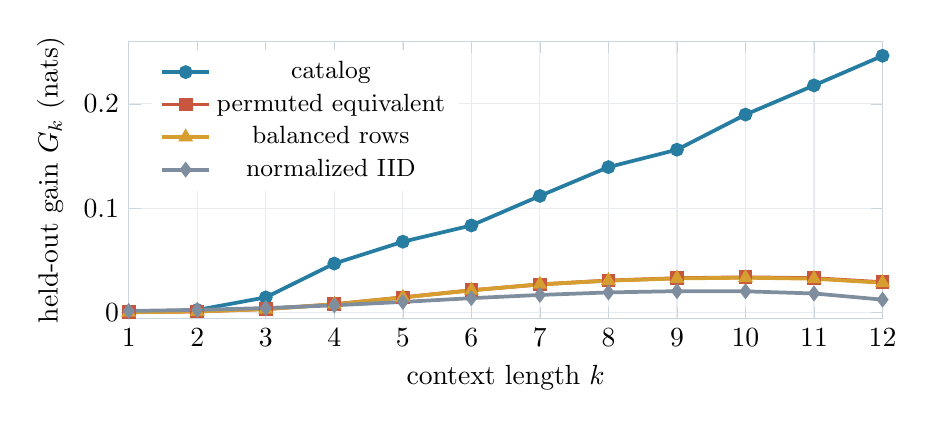
\begin{tikzpicture}
\begin{axis}[
  width=0.92\linewidth,
  height=5.1cm,
  xmin=1,xmax=12,
  ymin=-0.006,ymax=0.26,
  xtick={1,...,12},
  xlabel={context length $k$},
  ylabel={held-out gain $G_k$ (nats)},
  axis line style={draw=RuleGray},
  tick style={draw=RuleGray},
  grid=major,
  grid style={draw=RuleGray!45},
  legend style={draw=none,fill=white,font=\small,at={(0.03,0.97)},anchor=north west},
  every axis plot/.append style={line width=1.35pt,mark size=1.8pt}
]
\addplot[color=SignalBlue,mark=*] coordinates {
  (1,0) (2,0.002199) (3,0.014261) (4,0.046758) (5,0.067719) (6,0.083317)
  (7,0.111679) (8,0.139350) (9,0.156044) (10,0.189766) (11,0.217803) (12,0.246238)};
\addlegendentry{catalog}
\addplot[color=SoftRed,mark=square*] coordinates {
  (1,0) (2,0.000769) (3,0.003064) (4,0.007671) (5,0.014282) (6,0.021096)
  (7,0.026712) (8,0.030468) (9,0.032666) (10,0.033561) (11,0.032705) (12,0.028802)};
\addlegendentry{permuted equivalent}
\addplot[color=WarmGold,mark=triangle*] coordinates {
  (1,-0.000003) (2,0.000708) (3,0.002971) (4,0.007537) (5,0.014179) (6,0.021047)
  (7,0.026773) (8,0.030327) (9,0.032457) (10,0.033154) (11,0.032177) (12,0.028267)};
\addlegendentry{balanced rows}
\addplot[color=MidnightBlue!55,mark=diamond*] coordinates {
  (1,0.001222) (2,0.002269) (3,0.004021) (4,0.006644) (5,0.009901) (6,0.013521)
  (7,0.016600) (8,0.019033) (9,0.020236) (10,0.020074) (11,0.018017) (12,0.012087)};
\addlegendentry{normalized IID}
\end{axis}
\end{tikzpicture}
\caption{Order-$28$ context sweep.  Catalog representatives become increasingly predictable, while permuted equivalents track the balance-only control.  Error intervals are omitted because they are smaller than the markers at this scale; numerical intervals are archived with the results.}
\label{fig:sweep}
\end{figure}

The context sweep in \cref{fig:sweep} connects the experiment back to the proofs.  At $k=1$, catalog and permuted Hadamards attain exactly $G_1=0$, as \cref{thm:onestep} requires.  For orders $24$ and $28$, the catalog-minus-permuted interval is positive for every $k=2,\ldots,12$.  The gap grows with context, while the permuted and balanced curves remain nearly superposed.  At order $28$, unseen-context rates remain negligible through $k=12$, so the divergence is not a sparse-context illusion.  At orders $16$ and $20$, by contrast, high-$k$ unseen rates exceed $80\%$; their qualitatively similar curves are not used for broad claims.

Small residual contrasts below $0.001$ nats occur at isolated order-$28$ values $k=10,11$.  They were found in an exploratory twelve-context sweep, are not corrected for simultaneous testing, and do not reproduce consistently across $k$ or order $24$.  They are neither practically meaningful nor evidence for an invariant law.

\takeaway{The experiment does not say that Hadamard matrices lack local structure.  It says something more precise: the strong structure visible to a short row-wise reader belongs mainly to how the catalog representative is written.}

\section{Why this is the right first note}

The result resolves the first fork in the larger narrative.  Global order is exact: orthogonality, normalization, and balance are mathematical constraints.  Entrywise readability is conditional: the permuted signal collapses to the balance baseline, while the catalog coordinate convention exposes a transferable signal.  The later question is therefore not simply whether a signal exists, but whether a representation-resilient summary can distinguish branches that belong to a complete whole.

That qualification is useful rather than disappointing.  Exact search algorithms also choose coordinates, normalize partial objects, and break symmetries.  A representation-dependent predictor may help if its training and search conventions match.  It must, however, order branches rather than certify impossibility.

\begin{proposition}[Branch ordering preserves completeness]\label{prop:search}
Consider a finite exact search tree in which pruning occurs only through a sound infeasibility predicate.  Reordering the children at any node using an arbitrary statistical score preserves completeness, provided every unpruned child remains available.
\end{proposition}

\begin{proof}
Reordering changes only the visitation order of the finite set of unpruned nodes.  Sound pruning removes no feasible leaf, and retaining every unpruned child leaves the reachable leaf set unchanged.  Therefore an exhaustive traversal still visits every feasible leaf.
\end{proof}

This proposition supplies the bridge to the next two experiments.  The second note replaces arbitrary serialized context with the evolving constraint state and predicts regional composition.  The third embeds that regional score in an exact solver and measures first-solution nodes and backtracks.  A poor predictor may slow the search, but it cannot make the search incorrect.

Several questions remain deliberately outside the present claim.  We have not isolated which catalog-selection step creates the sequential regularity; tested held-out construction families or orders; averaged uniformly over the full equivalence group; or shown an asymptotic bound on local information.  Nor have we shown a search speedup.  Those are the next links in the chain, and the present result tells us which chain is honest to pursue.

\section{Conclusion}

A Hadamard matrix can be rigid without being locally readable, and locally readable without that readability being invariant.  The key is to ask not only \emph{whether} a context predicts, but \emph{under which representation}.  Exact mathematics predicts neutrality at one step and balance-induced dependence at longer scales.  Held-out experiments then reveal a much larger signal in catalog representatives, followed by its near-complete collapse under equivalence-preserving randomization.

So the signal is not nowhere; it is somewhere specific.  It lives in the representative.  That diagnosis motivates a better local object---the constraint summary of an unfinished region---while warning that a forecast about that object is not yet a forecast of eventual completability.

\paragraph{Reproducibility.}
The repository contains exact matrix verification, context extraction, the smoothed predictor, all 20 split/control repetitions, 80 leakage audits, raw result tables, bootstrap summaries, and environment metadata.  Raw catalog downloads are hash-recorded and regenerated from the cited source.

\bibliographystyle{plainnat}
\bibliography{references}

\end{document}
